% sec_intro.tex
\section{Введение}

\begin{figure}[h]
\centering
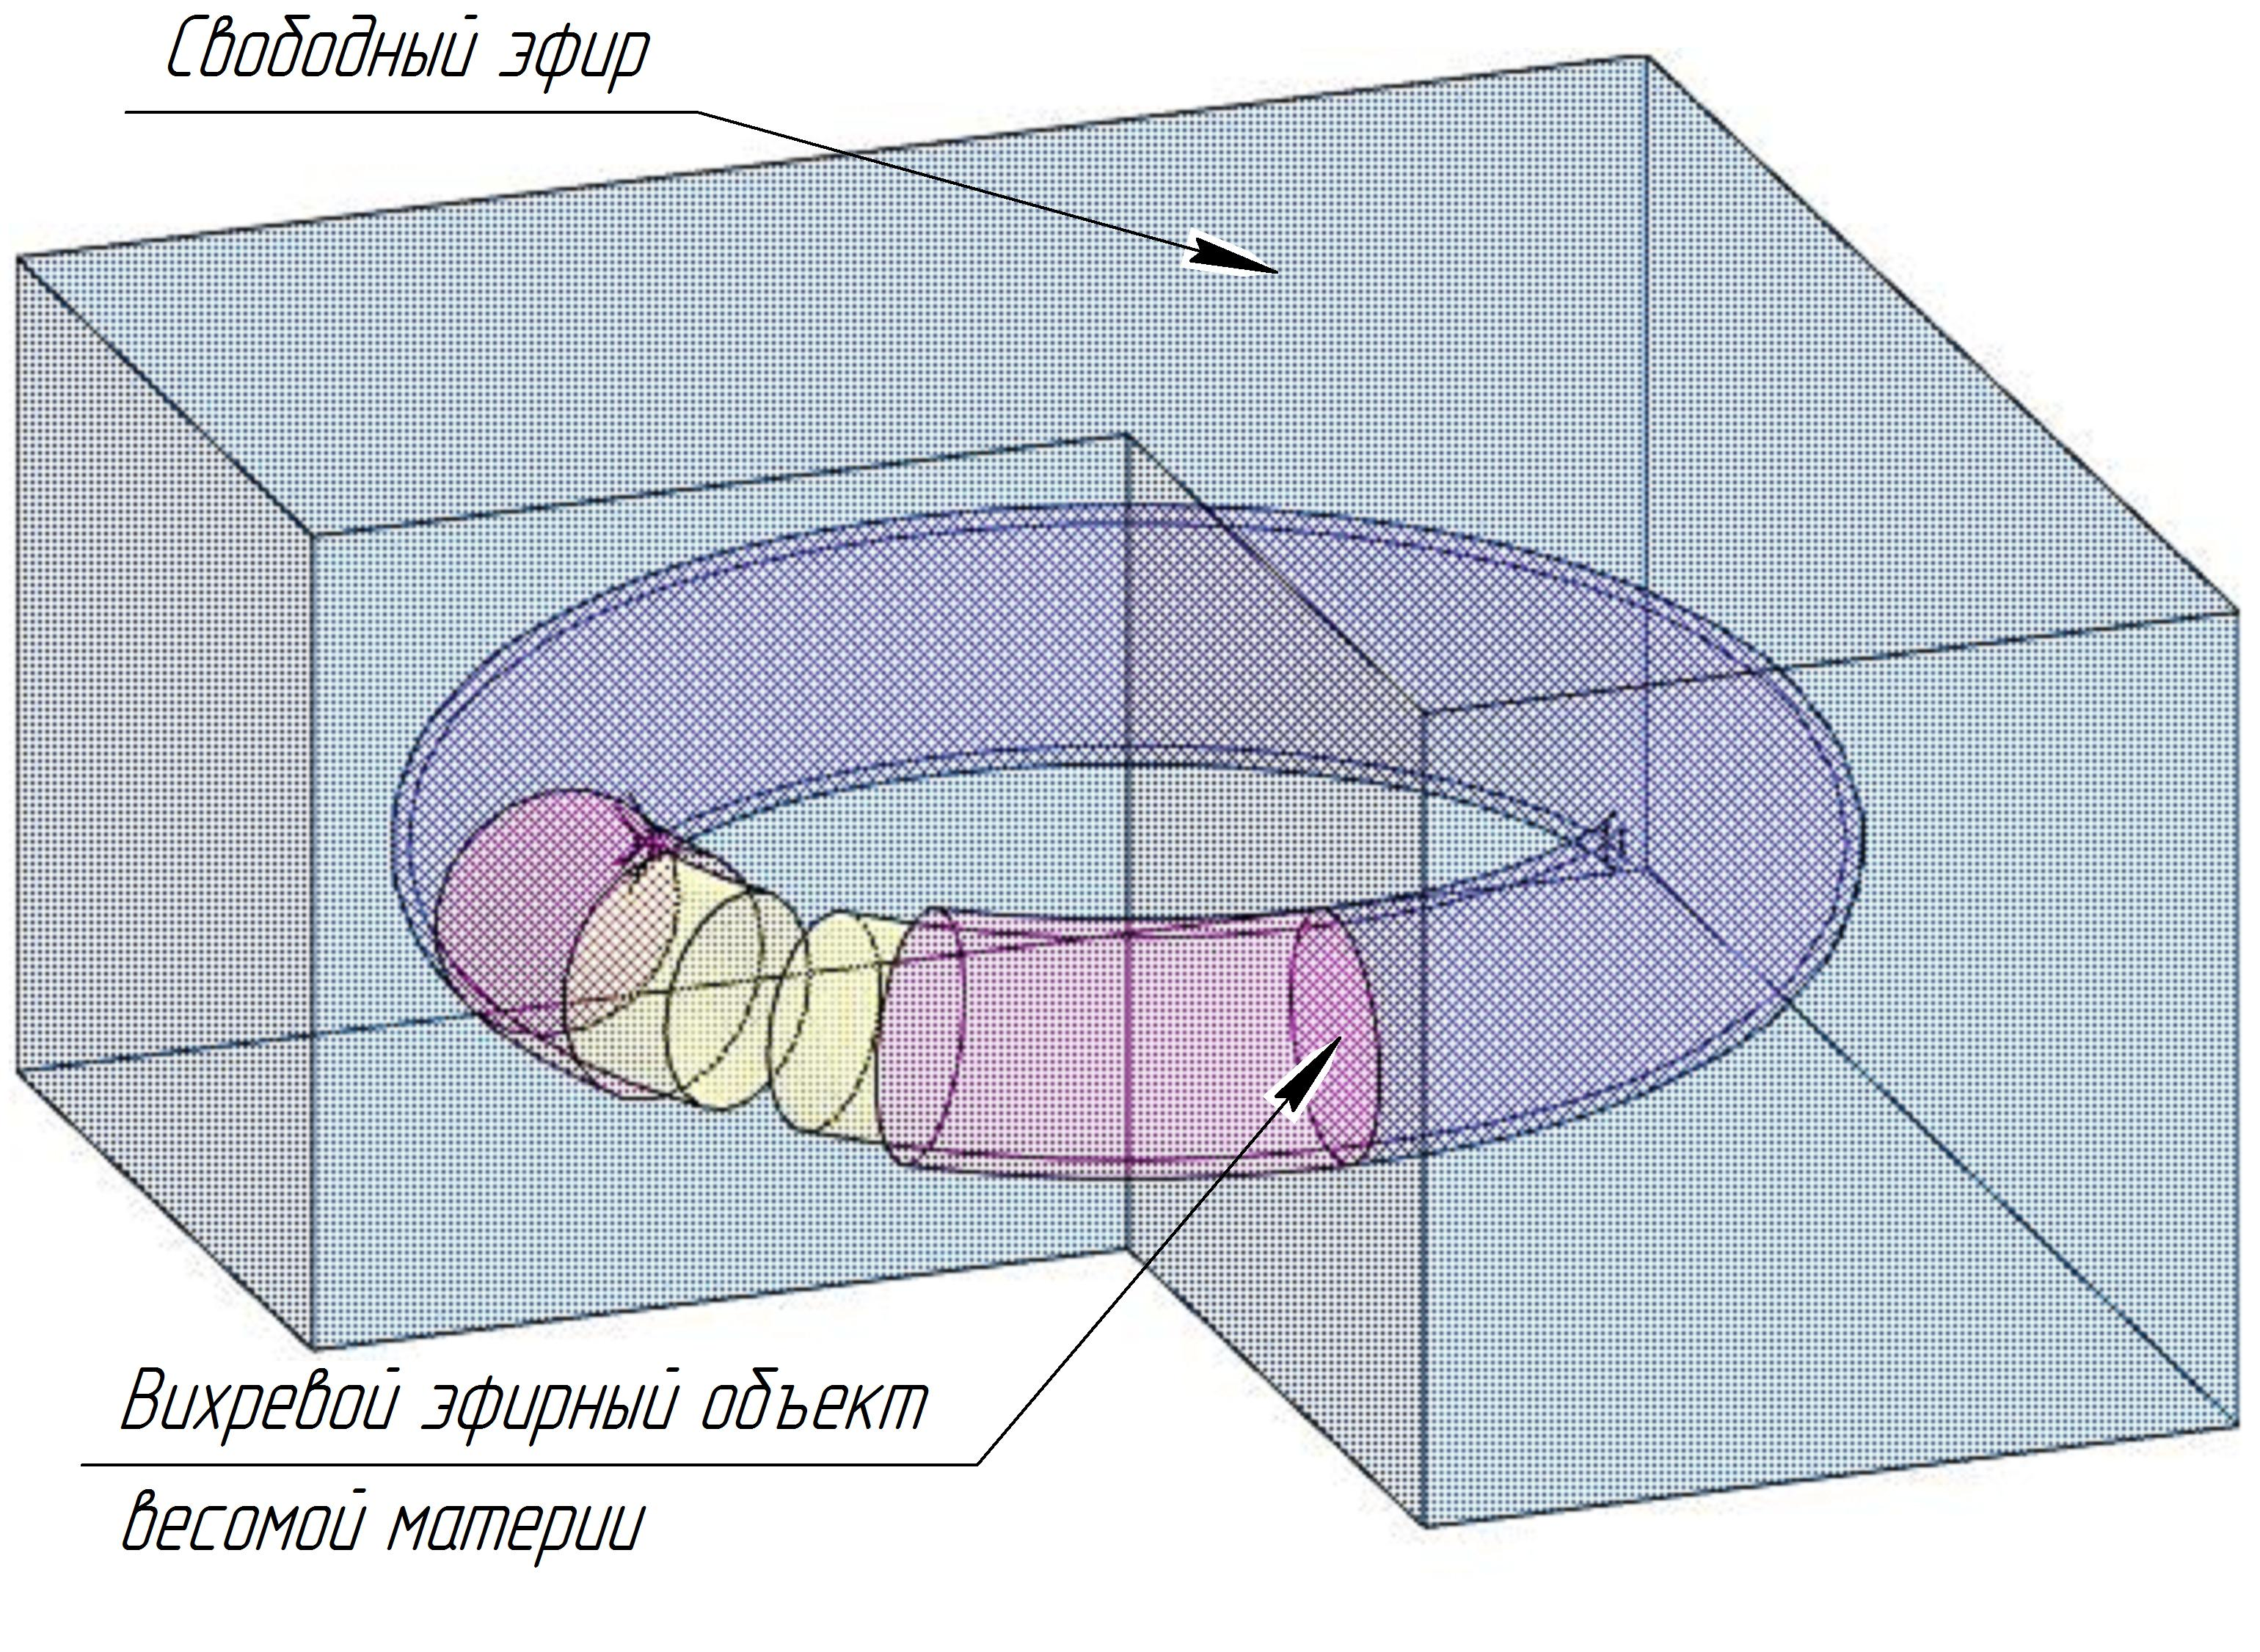
\includegraphics[width=0.4\textwidth]{images/bbbbb.png}
\caption{Схема вихревого объекта в среде свободного эфира.}
\label{fig:start}
\end{figure}

В процессе соударений частицы эфира находятся в состоянии непрерывного движения, которое осуществляется в форме \textbf{хаотического} и \textbf{направленного} движений. Результатом взаимодействия этих форм движения в рамках определённого физического сценария становится возможным осуществление локализации эфирных объектов в ограниченном пространстве. Из возможных пространственных комбинаций взаимодействия форм движения локализация осуществима в виде замкнутого направленного потока частиц эфира внутри объекта весомой материи, удерживаемого снаружи хаотически движущейся средой эфира. Как следствие, форма граничной поверхности топологически не предполагает существование каких-либо границ, так как в противном случае нарушается непрерывность процесса локализации объекта. Поверхности, обладающие таким свойством, — это \textbf{сфера} и \textbf{тороид}. \textbf{Эллипсоид}, являясь деформированной по трём осям сферой, в условиях \textbf{изотропности} хаотически движущейся среды эфира в качестве возможной формы граничной поверхности объектов весомой материи не рассматривается.

Процесс столкновений на граничной поверхности предполагает непрерывное повторение физического сценария его осуществления для каждой из частиц эфира по обе стороны поверхности, что предполагает взаимную обусловленность их кинетических параметров. Поток частиц эфира означает их направленное, одновременное, параллельное движение со скоростью, величина которой существенно превышает величину среднего значения хаотических пульсаций скорости каждой из частиц. Предположение о сферической форме граничной поверхности эфирного объекта и замкнутости потока частиц эфира внутри объекта, как показано на рисунке \ref{fig:spere}, с точки зрения кинетики его осуществления несостоятельно. Частицы в окрестности полюсов \(P\) совершают полный оборот значительно раньше экваториальных, что означает неминуемое разрушение потока и его трансформацию в хаотическую форму движения. Сами полюса \(P\) являются точками полной кинетической неопределённости, что указывает на несостоятельность предположения о сферичности граничной поверхности объектов весомой материи.

\begin{figure}[h]
\centering
\includegraphics[width=0.2\textwidth]{images/Sfere.png}
\caption{Несостоятельность сферической границы.}
\label{fig:spere}
\end{figure}

Таким образом, безальтернативным вариантом пространственной локализации замкнутого направленного потока частиц эфира является тороид, внутри которого частицы движутся по замкнутым спиральным, иными словами, \textbf{вихревым} траекториям. Анализ возможного движения частиц по пространственным траекториям, отличным от вихревой, неизменно приводит к кинетической неопределённости физического сценария осуществления локализации объекта, иначе говоря, к его разрушению. Вихревое движение частиц эфира, составляющих тело объекта весомой материи, и тороидальная форма его граничной поверхности сами по себе не являются определяющими факторами его локализации. Это условие необходимое, но недостаточное. Главным условием осуществления и дальнейшего существования объектов является присутствие внешней среды, состоящей из хаотически движущихся частиц эфира. Именно они — основные акторы этого процесса. Далее будем называть эту среду \textbf{Свободным эфиром}, а составляющие его частицы — \textbf{Амерами}.

\begin{figure}[h]
\centering
\includegraphics[width=0.3\textwidth]{images/АМЕР.png}
\caption{Амеры и свободный эфир.}
\label{fig:amers}
\end{figure}

Как видно из рисунка \ref{fig:start}, частицы эфира не являются бесконечно малыми точками сосредоточения массы, как это принято в классической молекулярно-кинетической теории газов; напротив, геометрия \textit{Амеров} в равной степени с их кинетикой движения влияет на осуществление вихревых эфирных локаций в условиях отсутствия иных прямых или косвенных внешних воздействий на этот процесс. Другими словами, \textbf{парные столкновения Амеров являются единственным физическим фактором, лежащим в основе осуществления объектов весомой материи, составляющих наблюдаемую Вселенную}. \textbf{Парность} столкновений является естественным следствием реактивного характера этого процесса и абсолютной упругости частиц эфира. Исходя из этой данности, являющейся, по сути, инвариантом, следует найти и сформулировать обоснованные, физически и логически непротиворечивые, причинно обусловленные \textbf{условия} и \textbf{критерии} осуществления направленного замкнутого потока частиц эфира в пределах пространственных границ вихря посредством их столкновений с хаотически движущимися частицами свободного эфира. Далее на основе полученных результатов составить физический сценарий автовоспроизводимого процесса осуществления объектов весомой материи с выявлением причинно-следственных последовательностей возникновения различных взаимодействий между ними.
